% ==============================================================================
%  $RCSfile: handbuch.tex,v $, $Revision: 1.14 $
%  $Date: 2003/09/19 19:50:36 $
%  $Author: birdy $
%
%  Description: Master Datei des Handbuchs
%
%  Last-Ispelled-Revision:
%
% ==============================================================================

\documentclass[a4paper,titlepage,11pt,german,twoside]{scrbook}

\clearpage
\makeatletter

%koma uses \chapter*, but we want to use \chapter
%  changed srcbook.cls-commands
\renewcommand\idx@heading{%
  \twocolumn
  \chapter{\indexname}\@mkboth{\indexname}{\indexname}
}

%Nummerierung soll net so eng aneinanderhaengen
\renewcommand*\l@section{\@dottedtocline{1}{1.5em}{3em}}

\makeatother


\usepackage{../styles/common}

\usepackage{verbatim}
\usepackage{shortvrb}

\usepackage{handbuch}

\usepackage{makeidx}
\makeindex

% subsubsections nummerieren
\setcounter{secnumdepth}{3}

\newcommand\version{Version 1.2\xspace}
%\newcommand\version{\today\xspace}

% header
\fancyhead{}
\fancyhead[LE,RO]{\slshape \company}
\fancyhead[LO,RE]{\slshape \leftmark}
\fancyfoot[LE,RO]{\thepage{}}
\fancyfoot[LO,RE]{\version}

\begin{document}

% title page
\thispagestyle{empty}
\hfill
\parbox{5.5cm}
{Universit�t Stuttgart\\
Studienprojekt A -- IML Browser\\
\company}

\vspace{3cm}

\begin{center}
  \Huge
  \textsf{Handbuch}\\
  \vspace{.5cm}
  {\Large\version}\\
  \vspace{3cm}
  \includegraphics[scale=.5]{../logo}
\end{center}
\newpage

\MakeShortVerb{\�}

\section*{Versionsgeschichte}

\begin{itemize}

\item Version 1.0 (08.04.2003)

  Zur Pr�fung im Kundenreview am 14.04.2003 - 16.04.2003.


\item Version 1.1 (22.04.2003)

  Korrekturen gem�� Kundenreview eingearbeitet.\\
  Diese Version der Spezifikation ging am 23.04.2003 
  zur Abnahme an den Kunden.

\end{itemize}

%%% Local Variables: 
%%% TeX-master: "spec"
%%% End: 


%===============================================================================
%
% Inhaltsverzeichnis
%
\newpage
\setcounter{tocdepth}{1}
\tableofcontents

%===============================================================================
%
% Einleitung
%
\chapter{Einleitung}
% ==============================================================================
%  $RCSfile: intro.tex,v $, $Revision: 1.1 $
%  $Date: 2003/02/13 03:15:14 $
%  $Author: schulzgt $
%
%  Description:
%
% ==============================================================================

\section{�ber dieses Dokument}
doc
\section{�ber GIANT}
giant


%===============================================================================
%
% Produkt�bersicht
%
\chapter{Produkt�bersicht}

In diesem Kapitel werden einige grundlegende Konzepte und
M�glichkeiten von GIANT vorgestellt und kurz beschrieben.

% ==============================================================================
%  $RCSfile: product.tex,v $, $Revision: 1.1 $
%  $Date: 2003/02/13 03:15:14 $
%  $Author: schulzgt $
%
%  Description:
%
% ==============================================================================

\section{IML-Teilgraphen}
\section{Anzeigefenster und Selektionen}
\section{Pins}
\section{Drei-Stufen-Konzept}

\chapter{Visualisierung des IML-Graphen}
Genaue Beschreibung der Visualisierung des Graphen in einem Anzeigefenster.
\section{Visualisierung von Knoten}
\section{Visualisierung von Kanten}
\section{Kantenknickpunkte}
\section{Minimap}

\chapter{Anfragesprache und Kommandozeilenaufruf}
\section{Beschreibung der Anfragesprache}
\section{Kommandozeilenaufruf}

\section{Das Projektverzeichnis}
\subsection{Verwaltungsdateien f�r Anzeigefenster}
\subsection{Verwaltungsdateien f�r IML-Teilgraphen}
\subsection{Verwaltungsdatei f�r Anfragen}
Kann er auch selber mittels Paste und Copy im Emacs machen.
\subsection{Identifikation der IML-Graph Datei}
\subsection{Grundlegendes Verhalten beim Speichern}


%===============================================================================
% 
% Technische Produktumgebung
%
\chapter{Technische Produktumgebung}

Hier wird die zum Betrieb von GIANT n�tige Hardware 
und die n�tige Software sowie die Installation von GIANT
auf Linux-Systemen beschrieben.

% ==============================================================================
%  $RCSfile: technical.tex,v $, $Revision: 1.4 $
%  $Date: 2003/02/21 17:55:53 $
%  $Author: schulzgt $
%
%  Description: Hier sind die Anforderungen an die Programmumgebung 
%  spezifiziert. Dazu geh�hren die verwendete Hard- und Software, sowie
%  Schnittstellen zu anderen Produkten.
%
% ==============================================================================

\section{Software}
Das Programm stellt an die installierte Software folgende Anforderungen:
\begin{itemize}
  \item Sun Solaris oder Linux Betriebssystem
  \item Bauhaus Tools
  \item Emacs oder vi Texteditor
\end{itemize}


\section{Hardware}
Das Programm l�uft auf SPARC Workstations und x86 kompatiblen PCs.
Im Folgenden sind die minimalen Hardwareanforderungen zur Arbeit mit kleinen 
und mittleren Projekten beschrieben. Bei gro�en Projekten ist ein Speicherausbau
von 2 GB und mehr empfehlenswert.

\subsection{Hardwareanforderungen SPARC}
\begin{itemize}
  \item UltraSPARC-II 300 MHz
  \item 512 MB Hauptspeicher
  \item 8 Bit Grafik mit einer min. Aufl�sung von 1024*786
  \item Maus mit mindestens 3 Tasten
\end{itemize}

\subsection{Hardwareanforderungen x86}
\begin{itemize}
  \item Pentium III 600 MHz
  \item 512 MB Hauptspeicher
  \item 8 Bit Grafik mit einer min. Aufl�sung von 1024*786
  \item Maus mit mindestens 3 Tasten
\end{itemize}

\section{Produkt-Schnittstellen}
Das Programm soll in die Bauhaus Suite integriert werden k�nnen.
Als Schnittstelle dient dabei die Bauhaus IML Bibliothek. Weiterhin
kann die Verwendung von Kommandozeilenparametern und der GQSL zur 
Integration in das vorhandene System genutzt werden.



%===============================================================================
%
% Konzepte und Begriffe
%
\chapter{Konzepte und Begriffe}

Dieses Kapitel f�hrt die f�r das Verst�ndnis dieses Handbuches und die
Benutzung von GIANT wichtigen Begriffe ein.
Eine tabellarische Beschreibung der einzelnen Begriffe findet sich
in der Spezifikation von GIANT, Kapitel Begriffslexikon.

% ==============================================================================
%  $RCSfile: konzepteundbegriffe.tex,v $, $Revision: 1.1 $
%  $Date: 2003/06/30 15:22:06 $
%  $Author: birdy $
%
%  Description:
%
%  Last-Ispelled-Revision:
%
% ==============================================================================


\section{�ber dieses Kapitel}

Dieses Kapitel f�hrt die f�r das Verst�ndnis dieses Handbuches und die
Benutzung von GIANT wichtigen Begriffe ein.

\section{Begriffe}

\begin{enumerate}

  \item{Anfrage (Query):}{ Eine Anfrage beschreibt einen Vorgang, bei dem
    �ber geeignete Kriterien IML-Konten und IML-Kanten aus dem IML-Graphen
    oder aus IML-Teilgraphen ausgew�hlt werden.}
  
  \item{Anzeigefenster (Visualization Window):}{ Ein Fenster in dem ein
    Teilgraph des IML-Graphen nach bestimmten Kriterien visualisiert
    ist. Jedem Anzeigefenster ist ein Anzeigeinhalt zugeordnet.}
  
  \item{Anzeigeinhalt (Window Content):}{ Eine \gq{virtuelle} Oberfl�che
    auf der die Objekte des visualisierten Teilgraphen (also
    Fenster-Knoten und Fenster-Kanten) angeordnet sind, d.h. r�umliche
    Layoutinformation zu allen Objekten des entsprechenden
    Anzeigefensters. Abh�ngig von der Zoomstufe ist jeweils nur ein
    bestimmter Teil des Anzeigeinhaltes sichtbar - der sichtbare
    Anzeigeinhalt.  Die Gr��e des Anzeigeinhaltes ist theoretisch
    unbegrenzt.}
  
  \item{Fenster-Kante (Window Edge): }{Die graphische Repr�sentation einer
    IML-Kante innerhalb eines Anzeigefensters.}
  
  \item{Fenster-Knoten (Window Node): }{Die graphische Repr�sentation
    eines IML-Knoten innerhalb eines Anzeigefensters.}
  
  \item{Graph-Kante (Graph Edge): }{Eine Kante des IML-Graphen welche
    Bestandteil eines IML-Teilgraphen ist.}
  
  \item{Graph-Knoten (Graph Node): }{Ein Knoten des IML-Graphen welcher
    Bestandteil eines IML-Teilgraphen ist.}
  
  \item{IML-Graph (IML Graph): }{Der IML-Graph, wie er von der Bauhaus
    Reengineering GmbH gestellt wird.  Auf diesen Graphen wird �ber
    das sogenannte Reflection Model zugegriffen.}
  
  \item{IML-Kante (IML Edge): }{Eine Kante des IML-Graphen.}
  
  \item{IML-Knoten (IML Node): }{Ein Knoten des IML-Graphen.}
  
  \item{IML-Teilgraph (IML Subgraph): }{Eine Menge �ber Knoten und Kanten
    des IML-Graphen, die so gestaltet ist, dass sie einen Teilgraphen
    des IML-Graphen darstellt.}
  
  \item{Kantenklasse (Edge Class): }{Die Einteilung der IML-Kanten des
    IML-Graphen in verschiedene Klassen, wie sie sich aus der
    IML-Graph-Bibliothek von Bauhaus ergibt.\\
    Innerhalb dieser Spezifikation ist der Begriff Kantenklasse so
    zu verstehen, dass jede IML-Kante eindeutig zu genau einer Kantenklasse
    geh�rt, eine Vererbungshierarchie existiert nicht. Die Zuordnung
    einer IML-Kante zu einer Kantenklasse wird durch die Knotenklasse
    des Start-Knotens und den Namen des Attributes
    (aus dem Bauhaus-IML-Graphen), welches die IML-Kante
    beschreibt, festgelegt. Jede vorkommende Kombination aus der
    Knoten-Klasse eines Start-Knotens und dem Namen eines Attributes,
    welches eine Kante beschreibt, ist somit eine eigene Kantenklasse}

  \item{Klassenmenge (Class Set): }{Eine durch die IML-Graph Bibliothek
    vorgegebene Zusammenfassung von Kantenklassen und Knotenklassen.
    Es kann mehrere Klassenmengen geben. Die selben Knotenklassen und 
    Kantenklassen k�nnen gleichzeitig zu mehreren Klassenmengen geh�ren.}

  \item{Knoten-Annotationen (Node Annotation): }{Eine textuelle
    Beschreibung zu einem bestimmten Knoten des IML-Graphen.}
  
  \item{Knotenklasse (Node Class): }{Die Einteilung der IML-Knoten des
    IML-Graphen in verschiedene Klassen, wie sie sich aus der
    IML-Graph-Bibliothek von Bauhaus ergibt.\\
    Im Sinne der Verwendung dieses Begriffes innerhalb dieser Spezifikation
    liegt den Knotenklassen keine Vererbungshierarchie zu Grunde, jeder
    IML-Knoten geh�rt also eindeutig zu genau einer Knotenklasse}
  
  \item{Layout (Layout): }{Die zweidimensionale r�umliche Anordnung von
    Fenster-Knoten und Fenster-Kanten innerhalb eines Anzeigefensters
    auf dem sogenannten Anzeigeinhalt.}
 
  \item{Reflektion (Reflection Model): }{Die Schnittstelle zum Zugriff
    auf den IML-Graphen.}
  
  \item{Schleife (Loop): }{Eine Kante mit identischem Start- und Zielknoten.
    Wird oft auch als Selbstkante bezeichnet.}
  
  \item{Selektion (Selection): }{Eine Auswahl von Fenster-Knoten und Fenster-Kanten 
    eines visualisierten Teilgraphen des IML-Graphen innerhalb eines
    Anzeigefensters.}
  
  \item{Sichtbarer Anzeigeinhalt (Visible Window Content): }{ Der Bereich
    des Anzeigeinhaltes eines Anzeigefensters, der zur Zeit sichtbar
    dargestellt wird.}
  
  \item{Zoomstufe (Zoom Level): }{ Dieser Faktor beschreibt die Gr��e des
    sichtbaren Anzeigeinhaltes.  Bei einer sehr niedrigen Zoomstufe
    (auch: weit weg gezoomt) ist ein gr��erer Teil des im
    Anzeigefenster visualisierten IML-Graphen sichtbar als bei einer
    hohen Zoomstufe (auch: sehr nach heran gezoomt).}
  
  \item{hervorheben (to highlight): }{Hervorheben bedeutet, dass in einem
    Anzeigefenster visualisierte Fenster-Knoten oder Fenster-Kanten
    z.B.\ durch eine farbige Umrahmung von anderen Fenster-Knoten oder
    Fenster-Kanten unterscheidbar gemacht werden.}
    
  \item{selektieren (to select): }{Selektieren beschreibt einen Vorgang
    �ber den der Benutzer, z.B.\ durch Anklicken von Fenster-Knoten
    oder Fenster-Kanten mit der Maus, eine Selektion aufbaut.}
    
\end{enumerate}


%===============================================================================
% 
% Tutorial
%
\chapter{Tutorial}
\label{Tutorial}

Dieses Kapitel beschreibt einige h�ufig vorkommende Analysen mit GIANT
und wie sie vom Benutzer ausgef�hrt werden k�nnen, um dem Benutzer einen
schnellen Start der Arbeit mit GIANT zu erm�glichen.\\
Eine genauere Beschreibung der Funktionen befindet sich in Kapitel \ref{Beschreibung der Funktionen}.

%===============================================================================
% 
% Beschreibung der Funktionen
%
\chapter{Beschreibung der Benutzeroberfl�che}
\label{Beschreibung der Funktionen}

Dieses Kapitel beschreibt, geordnet nach den in GIANT auftretenden Fenstertypen,
alle Buttons, Men�s und Funktionen. Dies ist als Nachschlagewerk �ber
alle Elemente der graphischen Benutzeroberfl�che (GUI) gedacht.

% ==============================================================================
%  $RCSfile: functions.tex,v $, $Revision: 1.5 $
%  $Date: 2003/07/03 12:41:00 $
%  $Author: birdy $
%
%  Description: 
%
%  Last-Ispelled-Revision:
%
% ==============================================================================


\section{�ber dieses Kapitel}    

Hier werden alle Elemente der Benutzeroberfl�che (Anzeigeelemente und
aktive Elemente wie Men�s etc.) von GIANT beschrieben.
Sofern nicht anders angegeben, sind hintereinander angegebene Elemente
(z.B. Listeneintr�ge) immer von links nach rechts oder von oben nach
unten beschrieben.
Alle Ausgaben sind immer linksb�ndig formatiert, sofern nicht anders
vermerkt.
Wichtige Informationen zur Persitzenz der Projekte in GIANT,
welche Informationen jeweils gespeichert werden, finden sich
im Abschnitt \ref{Project Persistenz der Projekte}.

\clearpage
\section {Main Window}

\begin{figure}[h!]
   \centering
   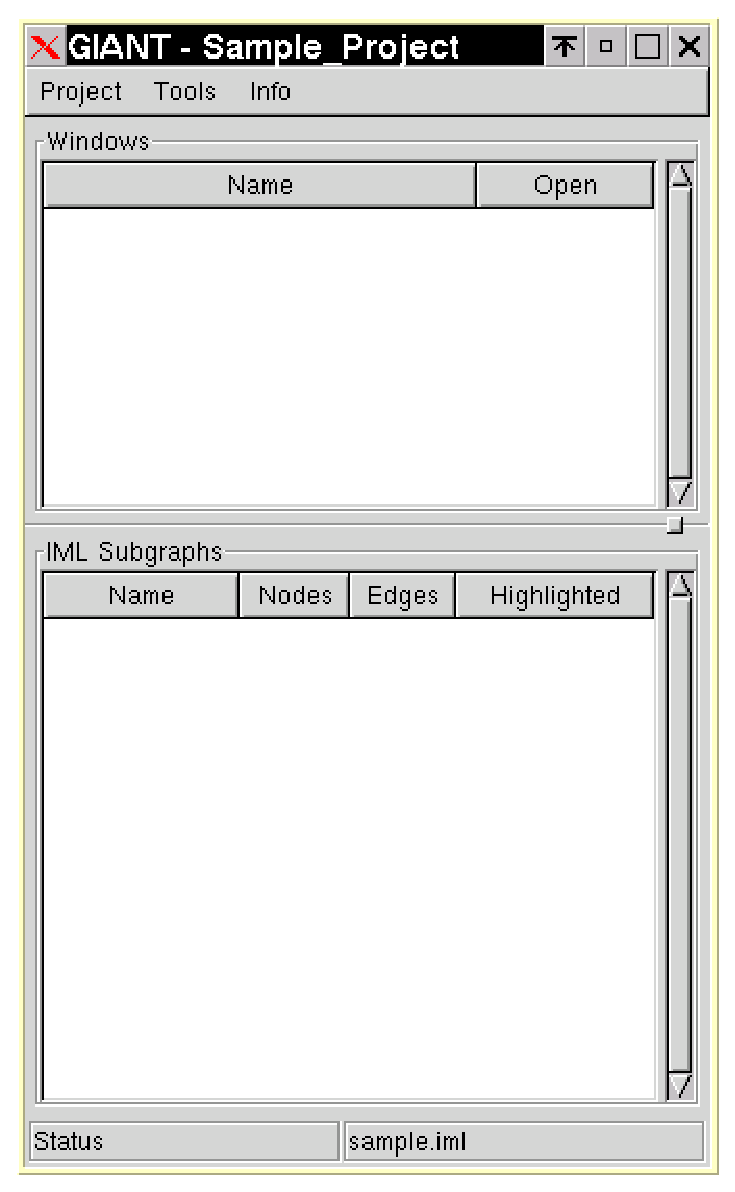
\includegraphics{gui/main_window}
   \caption{Main-Window}
   \label{Main-Window-Pic}
\end{figure}

%Erg�nzungen by Martin
Jede Instanz von GIANT hat genau ein Hauptfenster. \index{Hauptfenster}
Im Hauptfenster (siehe Abbildung \ref{Main-Window-Pic}) werden die
Anzeigefenster und
IML-Teilgraphen des aktuell ge�ffneten Projektes (siehe  
\ref{Project Persistenz der Projekte}) in Listen angezeigt. 
�ber Popup-Men�s k�nnen IML-Teilgraphen
und Anzeigefenster manipuliert werden.

Im Fenster befinden sich zwei Listen, Window List (2 Spalten), und
Subgraph List (4 Spalten).


  \subsection {Kopfzeile}
  In der Kopfzeile wird \gq{GIANT - <Projektname>} dargestellt.
 
  \subsection {Men�leiste (Main Window)}
  In der Men�leiste befinden sich folgende Eintr�ge:

    \subsubsection {Untermen� Project} \label{Main-Window-Project}
      \begin{enumerate}
         \item {New Project}\\
	 
	 Hiermit wird ein neues Projekt angelegt. Ein eventuell bereits ge�ffnetes
	 Projekt wird dabei geschlossen, wobei �nderungen auf Nachfrage 
         vorher gespeichert werden.

	 \begin{itemize}
	 
    \item{GIANT zeigt den Standard-Filechooser-Dialog und fordert den
    Benutzer auf, eine vorhandene IML-Graph Datei auszuw�hlen.}
    
    \item{GIANT zeigt erneut den Standard-Filechooser-Dialog und fordert den
    Benutzer zur Eingabe des Namens der Projektdatei auf. Die Dateiendung wird sp�ter
    von GIANT automatisch gesetzt.}
    
    \item {Der Name der Projektdatei ist
    automatisch auch der Name f�r das Projekt. Das Verzeichnis der
    Projektdatei wird automatisch zum Projektverzeichnis. Existiert die eingegebene Projektdatei bereits, 
    erscheint eine Fehlermeldung.
    Existiert in dem Projektverzeichnis bereits eine andere Projektdatei, so 
    erscheint ebenfalls eine Fehlermeldung.}
    	\end{itemize}
    
         \item {Load Project}\\
	 
	 �ffnet ein GIANT Projekt. Ein eventuell bereits ge�ffnetes
         Projekt wird dabei geschlossen, wobei �nderungen auf Nachfrage 
         vorher gespeichert werden.
	 \begin{itemize}
	   \item {War vorher bereits ein Projekt offen, erscheint vorher eine
	   Abfrage, ob dieses gespeichert werden soll.}
	   \item {GIANT zeigt den Standard-Filechooser-Dialog und fordert
           den Benutzer zur Auswahl einer vorhandenen GIANT-Projektdatei auf.}
	 \end{itemize}
         \item {Save Project}
	 
	 Speichert ein Projekt in die Verwaltungsdateien im Projektverzeichnis
	 der neuen Projektdatei.
	 
         \item {Save Project As...}
	 
	 Speichert ein Projekt in die Verwaltungsdateien im Projektverzeichnis
	 der neuen Projektdatei unter neuem Namen.
	 
	 \begin{itemize}
	  \item{Der Benutzer gibt im Standard-Filechooser-Dialog 
             das neue Projektverzeichnis 
             und den Namen f�r die neue Projektdatei ein, die Dateiendung 
             wird sp�ter von GIANT automatisch gesetzt.}
	 \end{itemize}
	 
         \item {Quit}
	 
	 Beendet das Programm GIANT.
	 
      \end{enumerate}    
      
     \subsubsection {Untermen� Tools}  \label{Main-Window-Tools}
       \begin{enumerate}
          \item {Delete Unreferenced Annotations}
	  
	  Es werden alle
          bestehenden Knoten-Annotationen des Projektes, f�r die es in
          Anzeigefenstern und IML-Teilgraphen keine Fenster-Knoten und
          Graph-Knoten gibt, gel�scht.
	  
          \item {Execute GSL Script}
	  
	  Mit diesem Men�punkt kann ein GSL Script ausgef�hrt werden.
	  Es erscheint der Skriptdialog, in den das Skript eingegeben
	  werden kann. Es ist auch m�glich, Skripte zu laden oder zu
	  speichern. Details hierzu finden sich unter \ref{GUI Anfragedialog}.
	  
        \end{enumerate}
        

    \subsubsection {Untermen� Info }  \label{Main-Window-Info}     
       \begin{enumerate}
          \item {About GIANT}
	  Dieser Men�punkt gibt ein Fenster mit Informationen zur
	  GIANT Programmversion und zu den Autoren aus.
        \end{enumerate}
     

  \subsection {Statuszeile}
  \label{Statuszeile}
  \index{Statuszeile}
  Die Statuszeile befindet sich ganz unten im Hauptfenster. In der
  Statuszeile werden Informationen zum aktuellen Zustand von GIANT
  dargestellt.

   \subsection {Window List}
  
   Im Hauptfenster befindet sich zuoberst eine Liste \gq{Window List}, welche
   alle Anzeigefenster des Projektes (offen und geschlossen anzeigt).
   Eine Beschreibung, was alles mit einem Fenster gespeichert wird,
   befindet sich in Abschnitt \ref{Project Persistenz der Projekte}.
   
   \subsubsection {Inhalt Window List}
   \label{WINDOW-LIST}
   
   Window List hat die Spalten \gq{Name} und \gq{Open}. In
   \gq{Name} wird der Name aller Anzeigefenster dargestellt, in
   \gq{Open} befindet sich entweder ein Strich-Symbol (Fenster
   nicht ge�ffnet) oder ein H�kchensymbol (Fenster ge�ffnet).
    
    \subsubsection {Popup-Men� Window List}
    
    
        Beim Rechtsklick auf Window List �ffnet sich ein 
        Popup-Men� mit folgenden Men�punkten:
        \label{WINDOW-LIST-POPUP}

        \begin{enumerate}
          \item New Window\\
	     Erzeugt ein neues leeres Fenster mit einem Standardnamen
	     (\gq{NewWindow}). 
          \item Open Window\\
	     �ffnet ein im Speicher vorhandenes, momentan geschlossenes Fenster.
          \item Close Window\\
	     Schlie�t ein vorhandenes Fenster, es kann wieder ge�ffnet werden.
	     Falls das Fenster noch nicht gespeichert wurde, wird eine
	     Sicherheitsabfrage durchgef�hrt, ob gespeichert werden soll.
          \item Save Window\\
	     Speichert ein Fenster im Projektverzeichnis.
          \item Delete Window\\
	     L�scht ein Fenster aus dem Projektverzeichnis, es wird auch aus der Window List gel�scht.
          \item Rename Window\\
	     �ndert den Namen eines Fensters, ein entsprechender Dialog erscheint.
        \end{enumerate}
    
  \subsection {Subgraph List}
  \label{GUI Subgraph List}
    
    Unter der Window List befindet sich eine Liste \gq{Subgraph List} mit
    allen IML-Teilgraphen des Projektes.
   
    \subsubsection {Inhalt Subgraph List} 
    
      Subgraph List hat die folgenden Spalten:
      \begin{enumerate}
        \item Name
        \item Nodes
        \item Edges
        \item Highlighted
      \end{enumerate}
    
      In der Spalte Name stehen die Namen der existierenden IML-Teilgraphen,
      in Nodes die Anzahl der Graph-Knoten des jeweiligen IML-Teilgraphen, 
      in Edges die Anzahl der Graph-Kanten und in Highlighted befindet sich
      ein K�stchen in der
      Farbe, die f�r die Hervorhebung des IML-Teilgraphen verwendet wird
      (siehe hierzu auch \ref{hervorheben von Knoten und Kanten}).
      Bei nicht hervorgehobenen IML-Teilgraphen wird dieses K�stchen
      nicht angezeigt.

    
    \subsubsection {Popup-Men� Subgraph List}
    \label {Popup-Men� Subgraph List}
      Bei einem Rechtsklick auf Subgraph List �ffnet 
      sich ein Popup-Men� mit folgenden Men�punkten:
        \label{SUBGRAPH-LIST-POPUP}
        \begin{enumerate}
          \item Highlight (Men�)
            \begin{enumerate}
              \item Color 1
              \item Color 2
              \item Color 3\\
	      Mit diesen drei Men�punkten kann der angew�hlte IML-Teilgraph
	      in allen Fenstern in der ausgew�hlten Farbe markiert werden.
            \end{enumerate}
          \item Unhighlight In All Windows\\
	     Mit diesen drei Men�punkten kann der angew�hlte IML-Teilgraph
	      in allen Fenstern wieder entf�rbt werden, die Markierung also
	      entfernt werden.
          \item Copy IML Subgraph\\
	     Mit diesem Men�punkt kann ein IML-Teilgraph kopiert werden.
	     Ein Dialog zur Eingabe des neuen Namens erscheint.
	  \item Insert IML Subgraph
	     ??????????????? % Wie funktioniert das?
          \item Delete IML Subgraph
	     Mit diesem Men�punkt kann ein IML-Teilgraph nach Sicherheitsabfrage
	     gel�scht werden.
	  \item Create Window Selection % OK
	     Mit diesem Men�punkt kann aus einem IML-Teilgraphen eine Fensterselektion
	     erzeugt werden.
          \item IML Subgraph Set Operation 
        \end{enumerate}   
        

\clearpage
\section {Anzeigefenster} \label{GUI Anzeigefenster}
\index{Anzeigefenster}

  \begin{figure}[!htbp]
     \centering
     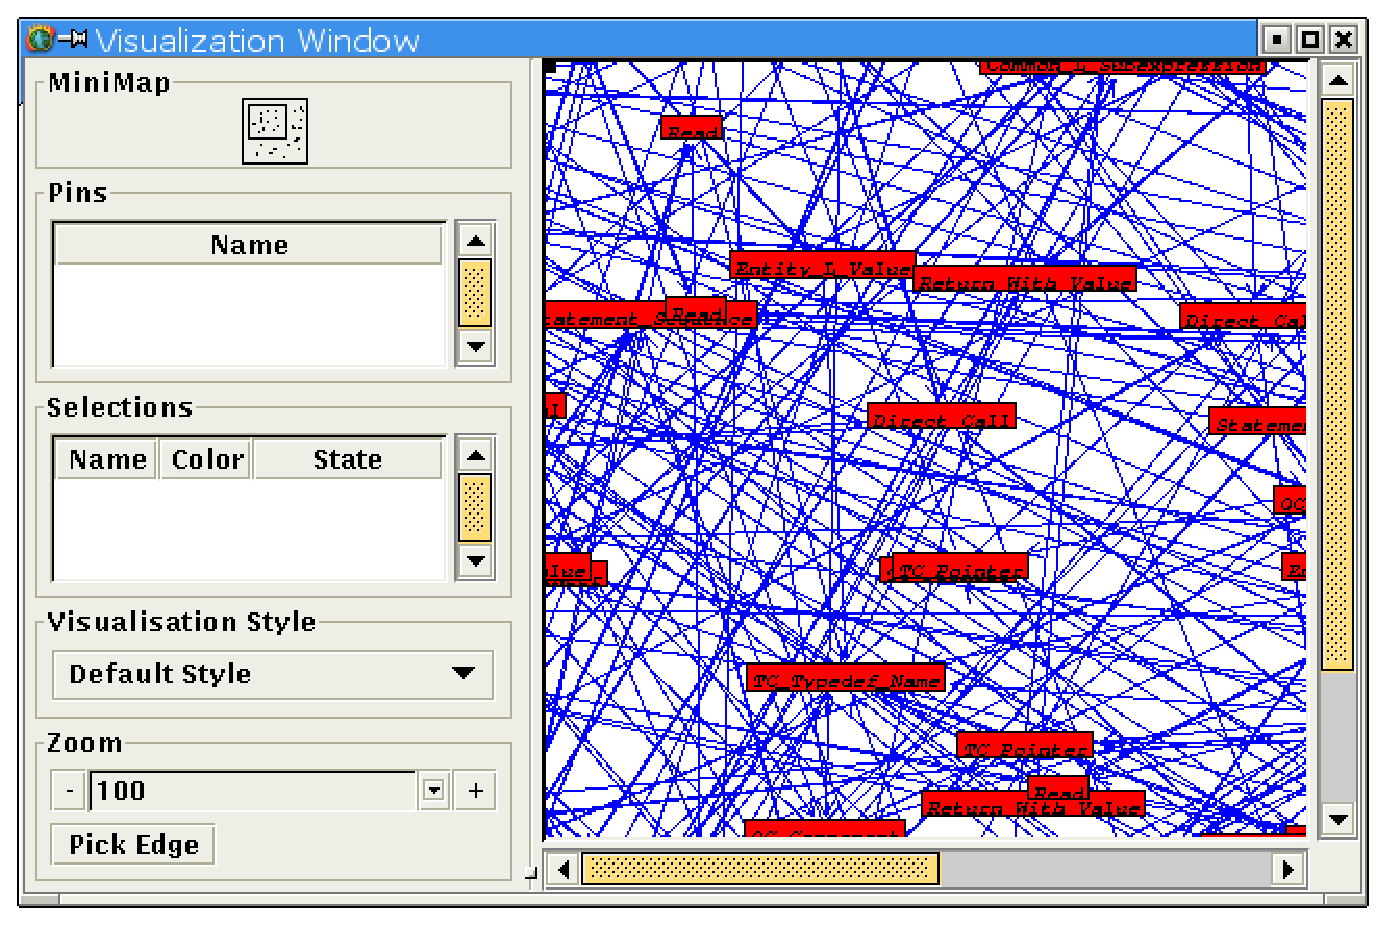
\includegraphics[width=16cm]{gui/visualization_window}
     \caption{Graph-Window}
     \label{Graph-Window-Pic}
  \end{figure}

  Im Programm kann es mehrere Anzeigefenster 
  (siehe Abbildung \ref{Graph-Window-Pic}) geben. 
  

  In Anzeigefenstern (Visualization Windows) werden Teile des IML-Graphen
  visualisiert.  Sie erscheinen im gro�en quadratischen rechten Teil
  (\gq{Vis Pane}) des Fensters. Die Vis Pane enth�lt den Anzeigeinhalt
  des Fensters.  Im linken Viertel des Fensters, der Toolbar
  (\gq{Vis Toolbar}) befinden sich untereinander die
  MiniMap, Pinliste, Selektionsliste, die Stilauswahl-Combobox und die
  Zoom-Kontrolle. 
  \index{Zoom-Kontrolle}
  \index{Visualisierungsstile!Stilauswahl-Combobox}

 \subsection {MiniMap} \label{GUI Minimap}
 \index{Minimap} 
 
 In der MiniMap wird der Anzeigeinhalt verkleinert dargestellt,
 der Graph wird jedoch nur durch einen grauen Kasten repr�sentiert,
 Knoten sind nicht sichtbar. Die MiniMap wird von einem Rahmen
 umschlossen. Der sichtbare Anzeigeinhalt wird durch einen kleineren
 Rahmen repr�sentiert, der innerhalb der MiniMap durch Mausklicks
 versetzt werden kann. Je nach Zoomstufe ist dieser Rahmen gr��er
 oder kleiner. Wird der Rahmen versetzt, wird der sichtbare Anzeigeinhalt
 in der Vis Pane entsprechend angepasst (siehe auch UseCase 
 \ref{Verschieben des sichtbaren Anzeigeinhaltes �ber die Minimap}).

  \subsection{Visualisierung der Knoten}

    In der Vis Pane werden die Fenster-Knoten und Fenster-Kanten angezeigt.
    
    Wenn auf einem Fenster-Knoten mit der rechten Maustaste geklickt wird, 
    �ffnet sich folgendes Popup-Men�:
 
    \subsubsection{Node-Popup-Men�}\label{Node-Popup-Men�}
    \begin{enumerate}
      \item Show Node Info Window\\
          Zeigt ein Fenster mit Informationen zum Knoten
      \item Show Corresponding Source Code\\
          Zeigt den zum Knoten geh�renden Source Code in einem externen Editorfenster
      \item Move Node\\
          Gibt dem Nutzer die M�glichkeit, den Knoten zu verschieben.
	  Nach Auswahl dieses Men�punktes geht GIANT in den "Paste Mode", der
	  Fadenkreuzcursor wird sichtbar. Durch Klick mit der linken Maustaste
	  an eine Stelle des Fensters wird der Knoten an dieser Stelle eingef�gt.
      \item Annotation (Men�)
        \begin{enumerate}
          \item Add\\
	     Mit diesem Men�punkt l��t sich eine Annotation zu einem Knoten hinzuf�gen.
	     Der Knoten ist dann graphisch als annotiert gekennzeichnet.
	     \begin{itemize}
	        \item{Der Nutzer f�hrt einen Rechtsklick auf den Knoten aus, den er
		       annotieren will und w�hlt im Popup-Men� \gq{Annotation - Add} an}
	        \item{Im erscheinenden Knotenannotations-Dialog kann der Text der
		      Annotation eingegeben werden und mit OK best�tigt werden.}
		\item{Nach dem n�chsten Speichern des Projektes ist die Annotation
		      dauerhaft erstellt.}     
	     \end{itemize}
          \item Change\\
	      Mit diesem Men�punkt l��t sich eine Annotation eines Knotens �ndern.
	     \begin{itemize}
	        \item{Der Nutzer f�hrt einen Rechtsklick auf den Knoten aus, dessen
		      Annotation er �ndern will und w�hlt im Popup-Men� \gq{Annotation - Change} an}
	        \item{Im erscheinenden Knotenannotations-Dialog kann der neue Text der
		      Annotation eingegeben werden und mit OK best�tigt werden.}
		\item{Nach dem n�chsten Speichern des Projektes ist die Annotation
		      dauerhaft ge�ndert.}
	     \end{itemize} 
          \item Delete\\
	       Mit diesem Men�punkt l��t sich eine Annotation eines Knotens l�schen.
	       \begin{itemize}
	        \item{Der Nutzer f�hrt einen Rechtsklick auf den Knoten aus, dessen
		      Annotation er l�schen will und w�hlt im Popup-Men� \gq{Annotation - Delete} an}
	        \item{Nach dem n�chsten Speichern des Projektes ist die Annotation
		      dauerhaft gel�scht.}
	     \end{itemize} 
          \end{enumerate}
      \label{Change Node Annotation}
      \label{Delete Node Annotation}
    \end{enumerate}
    
    Wenn in der Vis Pane mit der rechten Maustaste auf eine Stelle
    geklickt wird, an der kein Fenster-Knoten liegt, �ffnet sich das folgende
    Popup-Men�. Die Eintr�ge dieses Men�s sind auch im Node-Popup-Men�
    (siehe \ref{Node-Popup-Men�}) sichtbar.

    \label{Empty Vis Pane Right click}
    \begin{enumerate}
      \item Make Room\\
        \begin{itemize}
         \item{Der Nutzer f�hrt einen Rechtsklick auf eine leere Stelle des
	 sichtbaren Anzeigeinhalts in einem Anzeigefenster durch und w�hlt im erscheinenden
	 Popup-Men� \gq{Make Room} an}
	 \item{GIANT zeigt in der Statuszeile im Hauptfenster 
               \gq{Select position in display window}.
                Der Benutzer gibt den Punkt um den herum die Fenster-Knoten (und damit
                automatisch auch die Fenster-Kanten) auseinander geschoben werden
                 sollen �ber den Fadenkreuzcursor vor.}
	 \item{GIANT zeigt einen Dialog an, in dem der Benutzer ausw�hlt, um welchen 
               Betrag die Fenster-Knoten auseinander geschoben werden sollen.
	       Der Benutzer w�hlt einen geeigneten Betrag aus und best�tigt mit OK. }	 
         \item{GIANT schiebt die Knoten entsprechend auseinander.}
        \end{itemize}
      \item New Pin\\
         Mittels dieses Men�punktes kann ein neuer Pin angelegt werden.
	 \begin{itemize} 
	     \item{Der Benutzer f�hrt einen Rechtsklick auf den Anzeigeinhalt eines
    		Anzeigefensters durch und w�hlt aus dem Popup-Men� 
    		(siehe \ref{Empty Vis Pane Right click}) den Eintrag \gq{New Pin} aus.
    		Der sp�ter erstellte Pin verweist dann auf die Stelle im Anzeigeinhalt,
    		auf die der Rechtsklick durchgef�hrt wurde.}
    	     \item{Der Benutzer gibt im aufgehenden Texteingabedialog einen
	        zul�ssigen Namen f�r den neuen Pin ein und best�tigt mit OK}
    	     \item{GIANT speichert die aktuelle Zoomstufe und die Position des sichtbaren
    		Anzeigeinhaltes in einem neuen Pin.}
	 \end{itemize}
    \end{enumerate}
    

  \subsection{Pins} \label{VIS-PANE-Pins}
  \index{Pins}

    In der Pinliste (\gq{Pin List}) k�nnen Pins festgelegt werden.

    Im Popup-Men� der Pinliste befinden sich folgende Men�punkte:
    
    \begin{enumerate}
      \item Focus Pin\\
            Mittels dieses Men�punktes kann der sichtbare Anzeigeinhalt gem�� den im Pin gespeicherten
            Informationen gesetzt werden.
      \item Delete Pin\\
            Mittels dieses Men�punktes kann der Pin aus der Pinliste gel�scht werden.
    \end{enumerate}

  \subsection{Selektionsauswahlliste} \label{Selektionsauswahlliste}
    Die Selektionsauswahlliste hat die Spalten \gq{Name} mit dem Namen der
    Selektion, \gq{Color} mit der Farbe der Selektion und \gq{State}
    mit dem Status der Selektion (eingeblendet oder ausgeblendet).

    Im Popup-Men� der Selektionsauswahlliste (\gq{Selection List}) befinden
    sich folgende Eintr�ge:

    \begin{enumerate}
      \item New Selection\\
      Mit diesem Men�punkt k�nnen neue, leere Selektionen angelegt werden.
       \begin{itemize}
	  \item{GIANT �ffnet einen allgemeinen Texteingabedialog}
	  \item{Der Benutzer gibt dort einen zul�ssigen Namen 
           (siehe \ref{afa Zulaessige Namen}) f�r die neue Selektion 
           ein und best�tigt mit OK.}
	  \item{Eine neue Selektion mit dem vorgegebenen Namen
           ist angelegt und erscheint in der Liste der Selektionen.
           Diese neue Selektion ist leer, sie hat also keine selektierten 
           Fenster-Knoten und Fenster-Kanten).}
        \end{itemize}
      \item Move Selection\\
     Mit diesem Men�punkt k�nnen Fenster-Knoten oder ganze Selektionen auf dem
     Anzeigeinhalt verschoben werden. Dieses Verschieben geschieht mittels
     \gq{Cut and Paste}.
     \begin{itemize}
      \item{Der Benutzer w�hlt die zu verschiebende Selektion oder den
       zu verschiebenden Fenster-Knoten aus (\gq{Cut}), indem er
       Einen Rechtsklick auf eine Selektion in der Selektionsauswahlliste
       durchf�hrt und im Popup-Men� \gq{Move Selection} ausw�hlt,
       oder einen Rechtsklick auf einen Fenster-Knoten durchf�hrt
       und im Popup Men� \gq{Move Node} ausw�hlt.}
      \item{GIANT geht in den \gq{Paste Modus} �ber und zeigt
       dies in der Statusleiste des Hauptfensters an.  Der Cursor wird,
       falls er �ber den sichtbaren Anzeigeinhalt eines Anzeigefensters
       bewegt wird, zum Fadenkreuz.
       Die Funktionalit�t zum Zoomen und Scrollen des Anzeigefensters
       bleibt weiterhin verf�gbar, die �brige Funktionalit�t von GIANT
       wird gesperrt.}
      \item{Der Benutzer klickt mit der linken Maustaste an eine
       beliebige Stelle innerhalb des sichtbaren Anzeigeinhaltes des
       Anzeigefensters.
       GIANT verschiebt die ausgew�hlten Fenster-Knoten an die gew�nschte
       Stelle. Die zuvor mit dem Fadenkreuzcursor vorgegebene Position entspricht
       jetzt der des Mittelpunktes eines die verschobene Selektion umspannenden
       Rechtecks.}
     \end{itemize}
      \item Show Selection % war: Fade In Selection      

      \item Show all % Neu gemaess Daniel Simon

      \item Hide Selection % war: Fade Out Selection

      \item Layout Selection

      \item Create New IML Subgraph From This Selection % 
      
      \item Highlight Selection (Men�)
        \begin{enumerate}
        \item Color 1
        \item Color 2
        \item Color 3
        \end{enumerate}
	
      \item Unhighlight Selection % OK
        
      \item Zoom To Make Selection Fill Window % OK
     
      \item Copy Selection
      
      \item Copy Selection Keeping Existing Layout % OK
      \item Copy Selection Changing Existing Layout % OK
      \item Delete Selection % OK
      \item Delete Nodes and Edges of Selection
      \item Selection Set Operation % Changed by Martin
      
    %  \item Set Layout Algorithm For Selection --- deleted by Philipp
      
    \end{enumerate}    


  \subsection{Stilauswahl-Combobox}
  \label{GUI Stilauswahl-Combobox}   

    In der Stilauswahl-Combobox (\gq{Style Chooser}) kann ein 
    Visualisierungsstil (siehe auch \ref{Config Visualisierungsstile})
    ausgew�hlt werden.

  \subsection{Zoom-Kontrolle} \label{GUI Zoom-Kontrolle}  

    Die Zoom-Kontrolle besteht aus folgenden Elementen:
    
  \begin{enumerate}
      \item Button \gq{-} % OK
      \item Combobox mit vorgefertigten Zoom-Werten und Eingabem�glichkeit % OK
      \item Button \gq{+} % OK
      \item Button \gq{Pick Edge} % OK
  \end{enumerate}    

  In der ComboBox zur Zoom-Kontrolle befindet sich
  neben den vorgegebenen Zoomstufen \index{Zoomstufe} noch der
  Eintrag \gq{Fit in Window}.

    \subsection{Scrollbars}
    \label{Scrolleisten}
    
    Mit den beiden Scrollbars am unteren und rechten Rand des Anzeigefensters
    kann der sichtbare Anzeigeinhalt gescrollt werden.

\clearpage
\section{Knoten-Informationsfenster} \label{Knoten-Informationsfenster}

    \begin{figure}[!htbp]
       \centering
       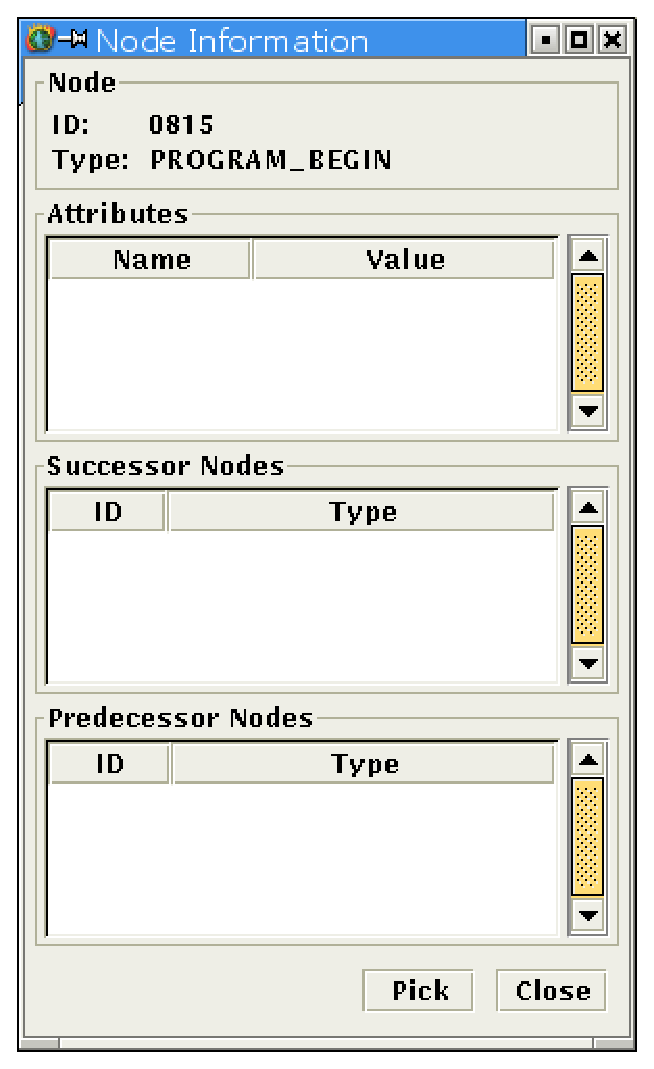
\includegraphics{gui/node_information_dialog}
       \caption{Node-Info-Window}
       \label{Node-Info-Window-Pic}
    \end{figure}

    In Knoten-Informationsfenstern (siehe Abbildung 
    \ref{Node-Info-Window-Pic}) 
    k�nnen n�here Informationen zu Fenster-Knoten angezeigt werden.
    
    Im Knoten-Informationsfenster wird die ID und die Knotenklasse des 
    vom Fenster-Knoten repr�sentierten IML-Knotens dargestellt,
    darunter befinden sich untereinander die drei scrollbaren 
    Listen \gq{Attributes}, \gq{Successor Nodes} und
    \gq{Predecessor Nodes}.
    
    Unter den drei Listen befinden sich nebeneinander zwei Buttons
    \gq{Pick} und \gq{Close}. 
    Pick dient zur Auswahl eines anderen Fenster-Knotens 
    mittels des Fadenkreuzcursors. Die Informationen zu dem ausgew�hlten
    Fenster-Knoten werden dann im Knoten-Informationsfenster dargestellt
    (siehe hierzu auch UseCase 
    \ref {Details zu Knoten in einem bestehenden Informationsfenster anzeigen}).
    
    \subsection{Liste Attributes}
    
    Die Liste Attributes enth�lt die Attribute des Knotens und hat
    zwei Spalten:
    
      \begin{enumerate}
        \item Name  (der Name des Attributes)
        \item Value (der Attributwert)
      \end{enumerate}
    
    \subsection{Liste Successor Nodes}
    
      Die Liste Successor Nodes hat eine Zeile f�r jede vom Knoten abgehende
      Kante mit zwei Spalten:
    
    \begin{enumerate}
      \item ID (die ID des Nachfolger-Knotens)  
      %Changed by Martin Class -> Type da sonst Inkonsistent zu Abbildung
      %Eigentlich h�tte die Grafik ge�ndert werden m�ssen
      \item Type (die Kantenklasse der abgehenden Kante)
    \end{enumerate}    

    \subsection{Liste Predecessor Nodes}
      
      Die Liste Predecessor Nodes hat eine Zeile f�r jede beim Knoten eingehende
      Kante mit zwei Spalten:

      \begin{enumerate}
        \item ID (die ID des Vorg�nger-Knotens)
        %Changed by Martin Class -> Type da sonst Inkonsistent zu Abbildung
        %Eigentlich h�tte die Grafik ge�ndert werden m�ssen
        \item Type (die Kantenklasse der eingehenden Kante)
      \end{enumerate}

\clearpage
\section{Skriptdialog} \label{GUI Anfragedialog}

    \begin{figure}[!htbp]
       \centering
       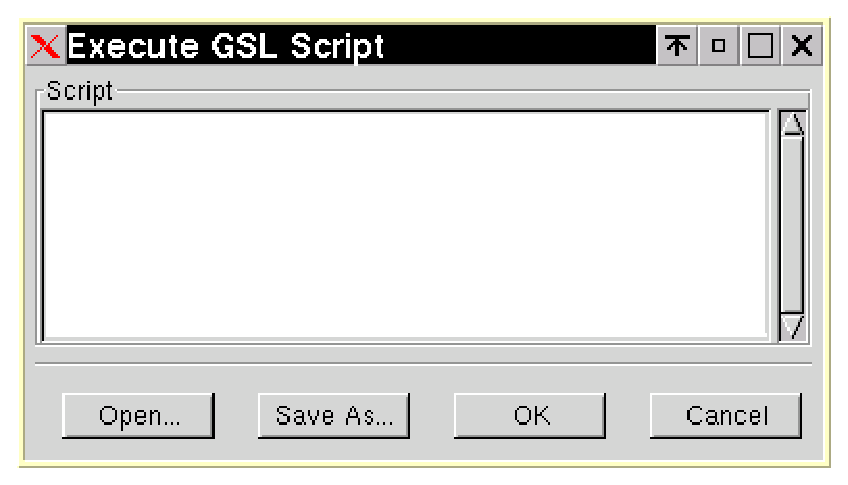
\includegraphics{gui/query_dialog}
       \caption{Skript-Dialog}
       \label{Skript-Dialog-Pic} 
    \end{figure}

Der Skriptdialog \gq{Query Dialog} (siehe Abbildung \ref{Skript-Dialog-Pic})
hat zuoberst ein Textfeld \gq{Query Text},
in das ein GSL Skript eingegeben werden kann.

Unter Query Text befinden sich folgende Buttons:

      \begin{enumerate}
        \item Open...
        \item Save As...
        \item OK
        \item Cancel
      \end{enumerate}
      
\clearpage
\section{Allgemeiner Texteingabedialog}
\label{DIALOG-WINDOW}

    \begin{figure}[!htbp]
       \centering
       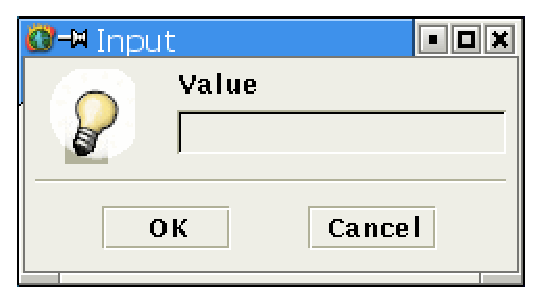
\includegraphics{gui/input_dialog}
       \caption{Dialog-Window}
       \label{Dialog-Window-Pic}
    \end{figure}

Ein allgemeiner Texteingabedialog ist ein Fenster Dialog Window 
(siehe Abbildung \ref{Dialog-Window-Pic}) mit dem
Titel \gq{Input}. Im Fenster ist ein einzeiliges Textfeld
mit einem Prompt-Text, zwei Buttons mit den Beschriftungen \gq{OK}
und \gq{Cancel}.

%\clearpage
\section{Set-Operation-Dialog}
\label{Common-Set-Operation-Dialog}

    \begin{figure}[!htbp]
       \centering
       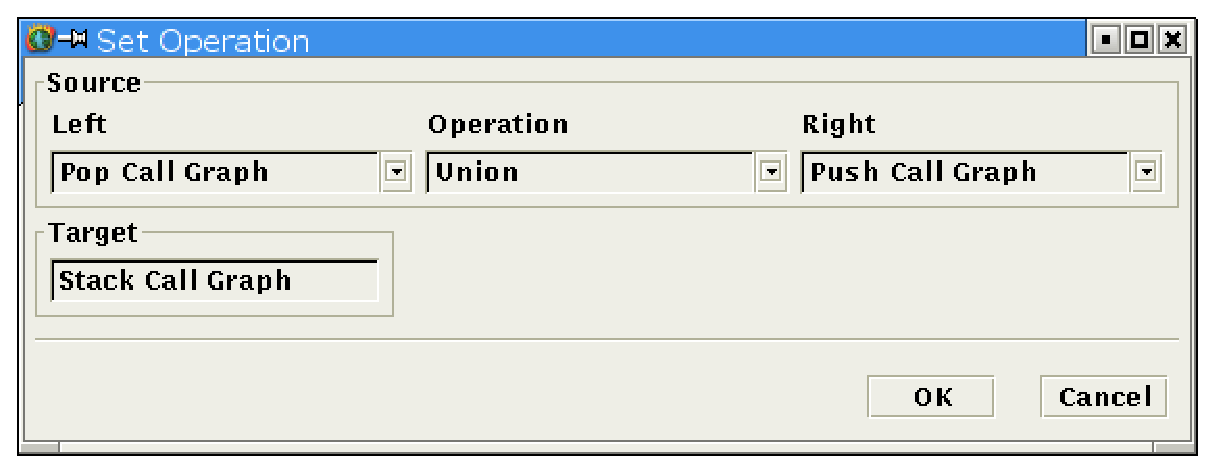
\includegraphics[width=16cm]{gui/set_operation_dialog}
       \caption{Set-Operation-Dialog}
       \label{Set-Operation-Dialog-Pic}
    \end{figure}


Der Set-Operation-Dialog (siehe Abbildung \ref{Set-Operation-Dialog-Pic}) 
dient dazu, Mengenoperationen �ber 
Selektionen und
IML-Teilgraphen durchzuf�hren.
Die Mengenoperation l�sst sich wie folgt beschreiben:\\
TARGET := LEFT\_SOURCE <op> RIGHT\_SOURCE \\


Bestandteile des Dialoges sind:
\begin {enumerate}

 \item LEFT\_SOURCE Combobox\\
 Soll eine Mengenoperation f�r Selektionen ausgef�hrt werden, so kann hier eine der
 Selektionen des entsprechenden Anzeigefensters ausgew�hlt werden.\\
 Bei einer Mengenoperation �ber IML-Teilgraphen, werden alle IML-Teilgraphen
 des Projektes angezeigt, von denen dann einer ausgew�hlt werden kann.
 
 \item <op> Combobox\\
 Mengenoperation, die ausgef�hrt werden soll; ausw�hlbar sind: Union, Difference oder Intersection.

 \item RIGHT\_SOURCE Combobox\\
 Soll eine Mengenoperation f�r Selektionen ausgef�hrt werden, so kann hier eine der
 Selektionen des entsprechenden Anzeigefensters ausgew�hlt werden.\\
 Bei einer Mengenoperation �ber IML-Teilgraphen, werden alle IML-Teilgraphen
 des Projektes angezeigt, von denen dann einer ausgew�hlt werden kann..
 
 \item TARGET Textfeld\\
 Name der neuen Selektion oder des neuen IML-Teilgraphen als Ergebnis
 der Mengenoperation.
 
 \item Buttons OK und Cancel\\
 Mit den beiden Buttons OK und Cancel l�sst sich die Operation starten bzw.
 der Dialog ohne Ausf�hren der Operation verlassen.
 
\end {enumerate}

 \clearpage
\section {Layoutalgorithmen Dialog}\label{Layoutalgorithmen-Dialog}

    \begin{figure}[!htbp]
       \centering
       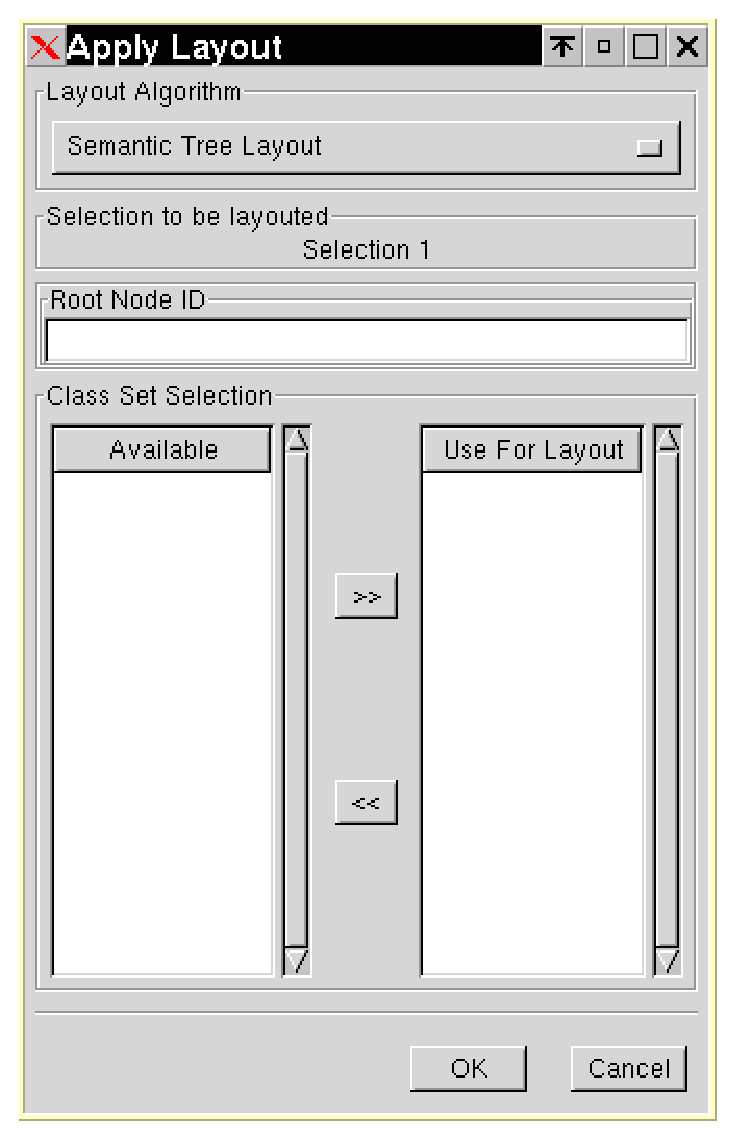
\includegraphics{gui/apply_layout_dialog}
       \caption{Layout-Algorithm-Dialog}
       \label{Layout-Algorithm-Dialog-Pic}
    \end{figure}

Der Layoutalgorithmen Dialog (siehe Abbildung \ref{Layout-Algorithm-Dialog-Pic}) 
bietet folgende M�glichkeiten:

\begin {enumerate}
 \item Auswahl des Layoutalgorithmus
 \item Ggf. Anzeige der zu layoutenden Selektion
 \item Ggf. Eingabefeld f�r die ID des Wurzelknotens bei Treelayouts
 \item {Eingabe der zu ber�cksichtigenden Klassenmengen bei semantischen Layouts,
 	Hierbei k�nnen mittels der Buttons \gq{>>} und \gq{<<} die 
        verf�gbaren
	definierten Klassenmengen zwischen den beiden
	Spalten \gq{Available} und \gq{Use For Layout} 
        hin und her geschoben werden.
	Nur Klassenmengen, die sich in der \gq{Use For Layout} Spalte befinden,
	werden f�r das Layout ber�cksichtigt.
        }
 \item OK Button
 \item Cancel Button
\end {enumerate}

\clearpage
\section{Dateneingabe}
Beschreibung von verschiedenen GUI Elementen zur Eingabe von Daten.

\subsection{Knoten-Annotations-Dialog}
\label{Knoten Annotations-Dialog}

    \begin{figure}[!htbp]
       \centering
       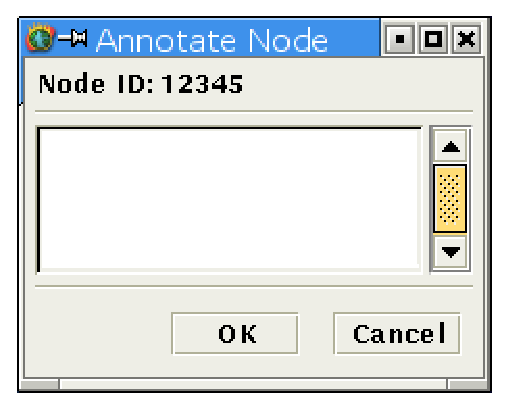
\includegraphics{gui/annotate_node}
       \caption{Node-Annotation-Dialog}
       \label{Node-Annotation-Dialog-Pic}
    \end{figure}
  
Der Knoten-Annotations-Dialog (siehe Abbildung 
\ref{Node-Annotation-Dialog-Pic}) besteht aus einem Fenster mit einem
Label, welches die ID des Knotens anzeigt, und einem Textfeld f�r den Annotationstext.
Mittels der beiden Buttons OK und Cancel k�nnen die �nderungen im
Textfeld �bernommen oder verworfen werden.  
\index{Knoten-Annotationen}


%  \clearpage
\subsection{Platz Schaffen-Dialog}
\label{Platz Schaffen-Dialog}

    \begin{figure}[!htbp]
       \centering
       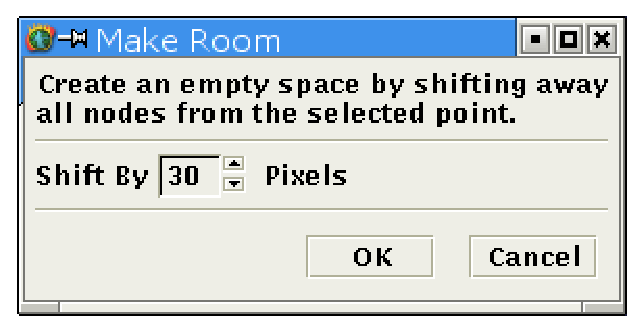
\includegraphics{gui/make_room}
       \caption{Make-Room-Dialog}
       \label{Make-Room-Dialog-Pic}
    \end{figure}

Im Dialogfenster Make Room (siehe Abbildung \ref{Make-Room-Dialog-Pic}) 
wird in einem Textfeld als Zahl 
eingegeben, um wie viel
Pixel die Fenster-Knoten an einer vorher markierten Stelle auseinandergeschoben 
werden sollen.
Mit dem Button OK kann best�tigt werden, mit dem Button Cancel abgebrochen werden.

\clearpage
\section{Ausgabe von Fehlermeldungen}
\label {GUI Ausgabe von Fehlermeldungen}

    \begin{figure}[!htbp]
       \centering
       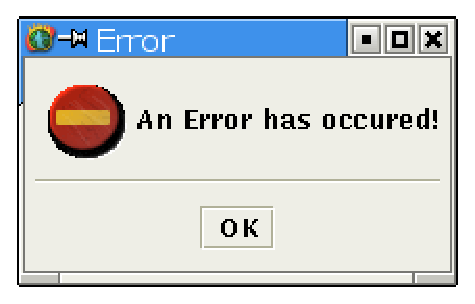
\includegraphics{gui/error_dialog}
       \caption{Error-Window}
       \label{Error-Window-Pic}
    \end{figure}

Ein allgemeiner Fehlerdialog (siehe Abbildung \ref{Error-Window-Pic}) 
ist ein Fenster \gq{Error Window}
mit dem Titel \gq{Error}. Im Fenster befindet sich ein Label zur
Ausgabe der Fehlermeldung und ein Button mit der standardm��igen 
Beschriftung \gq{OK}. 
F�r weitere Informationen zum allgemeinen Fehlerverhalten von GIANT siehe auch
Abschnitt \ref{afa Fehlerverhalten}.

\section{Sicherheitsabfrage}\label{Sicherheitsabfrage}
\index{Sicherheitsabfrage}

    \begin{figure}[!htbp]
       \centering
       
\includegraphics{gui/confirmation_dialog}
       \caption{Confirmation-Window}
       \label{Confirmation-Window-Pic}
    \end{figure}
    
Eine allgemeine Sicherheitsabfrage (siehe Abbildung \ref{Confirmation-Window-Pic}) 
ist ein Fenster (\gq{Confirmation Window}) mit dem
Titel \gq{Confirmation}. Im Fenster ist
ein Fragetext und ein Button mit der standardm��igen Beschriftung
Beschriftung \gq{Yes}, sowie ein Button mit der standardm��igen Beschriftung
\gq{No}. In dem Fragetext steht jeweils kontextabh�ngig 
die Information, die der  Benutzer zur Beantwortung der Sicherheitsabfrage
ben�tigt.

\clearpage

\section{Auswahl von Dateien}

  \subsection {Der \gq{Standard-Filechooser-Dialog}}
  \label {Standard-Filechooser-Dialog}

    \begin{figure}[!htbp]
       \centering
       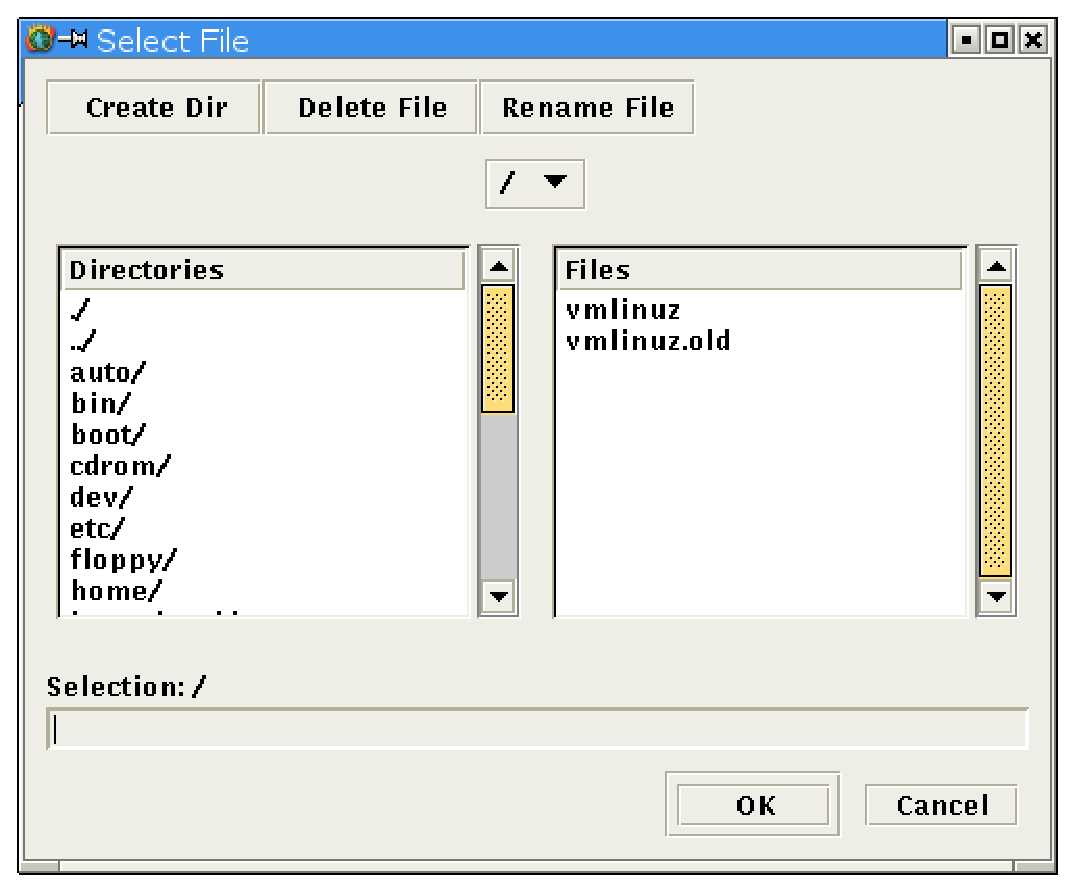
\includegraphics{gui/filechooser_dialog}
       \caption{Filechooser-Window}
       \label{Filechooser-Window-Pic}
    \end{figure}

Die Auswahl von Dateien (Laden/Speichern) passiert bei GIANT mittels
des Standard-Filechooser-Dialogs (siehe Abbildung \ref{Filechooser-Window-Pic}). 
Dieser Dialog ist Bestandteil der Widget-Bibliothek von GTK.


\section{Fadenkreuz-Cursor}
\label{Fadenkreuzcursor}
        Der Cursor verwandelt sich nach Auswahl bestimmter
        Funktionen (siehe z.B. UseCase \ref{Platz schaffen}) in ein Fadenkreuz.
        Durch Linksklick auf einen Fenster-Knoten oder eine 
        Fenster-Kante in einem Anzeigefenster  
        wird diese(r) f�r die jeweilige Funktion ausgew�hlt. 
        Der Fadenkreuz-Cursor wird auch zur Vorgabe von Positionen,
        an denen dann z.B. neue Fenster-Knoten eingef�gt werden,
        verwendet.
        Nach dem Linksklick  verwandelt
        sich der Fadenkreuz-Cursor wieder in den Standard-Cursor.
        Durch einen Rechtsklick bei aktivem Fadenkreuz-Cursor l�sst sich 
        die aktuelle Funktion abbrechen.


\section{Fortschrittsanzeige}
\label{GUI-Fortschrittsanzeige}
\index{Progressbar}


\label{Progressbar}
Es gibt in GIANT zwei M�glichkeiten zur Fortschrittsanzeige w�hrend
laufender Berechnungen.  Jede Progressbar ist mit \gq{The system is
busy. Please be patient.} beschriftet.

%\clearpage
\subsection{Progressbar-Runs}
\label{Progressbar-Runs}

     \begin{figure}[!htbp]
      \centering
      \includegraphics{gui/progressbar_busy}
      \caption{Progressbar-Runs}
      \label{Progressbar-Runs-Pic}
     \end{figure}

     Hierbei handelt es sich um ein Fenster mit einem sich bewegenden bzw. sich st�ndig 
     �nderndem Inhalt (z.B. ein Progress-Balken), so dass f�r den Benutzer erkennbar ist, 
     dass das System noch arbeitet 
     (beispielhafte Grafik siehe Abbildung \ref{Progressbar-Runs-Pic}).
  
%\clearpage
\subsection{Progressbar-Modal}
\label{Progressbar-Modale}      
     \begin{figure}[!htbp]
      \centering
      \includegraphics{gui/progressbar_cancel}
      \caption{Progressbar-Modal}
      \label{Progressbar-Modal-Pic}
     \end{figure}
     Der \gq{Progressbar-Modal}
     (siehe Abbildung \ref{Progressbar-Modal-Pic}) ist ein Fenster, 
     dass �ber den aktuellen Fortschritt
     einer Berechnung informiert, wobei der Gesamtaufwand unbekannt sein kann. 
     Hierzu wird kontinuierlich die Anzahl der schon bearbeiteten
     Datens�tze textuell ausgegeben, und, sofern bekannt, die Prozentzahl 
     der bereits
     bearbeiteten Datens�tze im Verh�ltnis zur gesamten Datenmenge.
     W�hrend dieser Dialog sichtbar ist, ist der Rest der GUI von GIANT
     gesperrt.
     Im Fenster existiert ein Button \gq{Cancel} \label{Progressbar-Modale-Cancel}, 
     mit dem eine laufende Berechnung abgebrochen werden kann.

%%% Local Variables: 
%%% TeX-master: "spec"
%%% End: 



%===============================================================================
% 
% Anfragesprache
%
\chapter{GIANT Scripting Language}
\label {GIANT Scripting Language}

Die F�higkeiten der GIANT Scripting Language (GSL) werden im Anhang 
\gq{GSL}, der Teil der GIANT Spezifikation ist, beschrieben.

\section{GSL-FAQ}
\subsection{Wie starte ich GSL?}
Zwei M�glichkeiten:

\begin{itemize}
  \item �ber Kommandozeile
  \item �ber Query-Dialog
\end{itemize}

Dar�berhinaus gibt es noch die M�glichkeit, vorgefertige Skripte �ber
die Men�s zu starten. 

\subsection{Mein Script bei if funktioniert nicht als condition}
So ist das auch nicht spezifiziert. Abhilfe:

\begin{verbatim}
  // ...
  +start_cond;
  if
    (is_script (b),
     {() set ('start_cond, b ())},
     {() set ('start_cond, b   )});
  if
    (start_cond,
    // ...
\end{verbatim}

Wichtig ist hier, dass beide Zweige als Skripte implementiert
sind. Siehe auch Frage \ref{if_eval}.

\subsection{If f�hrt immer beide Zweige aus}

Beispiel:

\begin{verbatim}
  if 
    (true,
     set ('a, 10),
     set ('a, 20))
\end{verbatim}

a ist jetzt 20 und nicht 10.

Der Grund liegt in der Auswertung: if ist auch ein GSL-Skript. Um ein
Skript auszuf�hren, werden zuerst die Parameter f�r dieses Skript
interpretiert und das Ergebnis dieser Interpretation dem Skript
�bergeben. Bei obigem Beispiel sind das true, 10 und 20, da die
Skripte \verb1set ('a, 10)1 und \verb1set ('a, 20)1 \gq{ausgef�hrt}
wurden. Nachdem true true ist, wird 10 ausgewertet, was zu 10 f�hrt.

Richtig ist deshalb:

\begin{verbatim}
  if 
    (true,
     {() set ('a, 10)},
     {() set ('a, 20)})
\end{verbatim}

Hier in den Zweigen nach der Auswertung und vor der \gq{Ausf�hrung}
von if Aktivierungsinformationen liegen. Und so wird nach der
Entscheidung, welcher Zweig ausgewertet werden soll, die
Aktivierungsinformationen zu Skripten ausgewertet.

%===============================================================================
% 
% Projektverwaltung
%
\chapter{GIANT Projektverwaltung}
\label{GIANT Projektverwaltung}

In diesem Kapitel wird beschrieben, wie persistente Arbeitsergebnisse
von GIANT strukturiert und gespeichert werden.
Arbeitsergebnisse sind z.B. vom Benutzer erzeugte Anzeigefenster
mit als Fenster-Knoten visualisierten IML-Knoten eines IML-Graphen.
Soweit f�r das Verst�ndnis von GIANT n�tig, sind auch Interna des
Programms festgehalten.

% ==============================================================================
%  $RCSfile: project.tex,v $, $Revision: 1.17 $
%  $Date: 2003/02/25 14:33:49 $
%  $Author: squig $
%
%  Description:
%
% ==============================================================================


%===================
\section {Persistenz �ber Projekte}

GIANT speichert persistente Informationen in so genannten Projekten.
\begin {enumerate}

  \item 
  Wird w�hrend des Betriebs von GIANT ein neues Projekt angelegt, so erh�lt 
  es automatisch eine Projektdatei.
  
  \item
  Ein Projekt besteht aus einem Verweis auf eine IML-Graph-Datei, auf die sich
  die gespeicherten Informationen beziehen, sowie aus den gespeicherten 
  Informationen f�r IML-Teilgraphen, Anzeigefenster und Knoten-Annotationen.
 
  \item
  Jedes Projekt hat einen vom Benutzer definierbaren Namen, dieser Name 
  entspricht dem Namen der Projektdatei und wird innerhalb des IML-Browsers 
  angezeigt.

  \item
  Der Name eines bereits angelegten Projektes kann mit den Mitteln von 
  GIANT nicht ge�ndert werden (au�er dadurch, dass  man das Projekt unter 
  neuem Namen neu speichert). 

  \item
  Der Benutzer kann beliebig viele Projekte anlegen.
  
  \item
  In GIANT darf immer nur ein Projekt gleichzeitig ge�ffnet sein. 
  
  \item
  W�hrend der Arbeit mit GIANT kann jederzeit ein Projekt geladen oder ein
  neues Projekt angelegt werden. 
  Voraussetzung hierf�r ist allerdings, dass dies 
  in der Reflektion zum IML-Graphen unterst�tzt wird.
  
  \item
  GIANT wei� nicht, ob ein geladenes Projekt gegen�ber den f�r das Projekt
  in der Projektdatei und in den Verwaltungssdateien gespeicherten 
  Informationen modifiziert wurde oder nicht.

\end {enumerate}


  \subsection {Das Projektverzeichnis}
  \begin {enumerate}

    \item  
    S�mtliche Dateien, die die Informationen f�r ein Projekt enthalten,
    befinden sich in diesem Verzeichnis. 

    \item
    In einem Projektverzeichnis darf nur ein Projekt abgelegt werden.
    
  \end {enumerate}    


  \subsection {Die Projektdatei}
  \begin {enumerate}

    \item
    Die Projektdatei liegt als XML-Datei vor.

    \item
    Die Projektdatei befindet sich im Projektverzeichnis und enth�lt 
    Informationen, die zur Identifikation des zu einem Projekt geh�renden 
    IML-Graphen n�tig sind. 
  
    \item
    Der Name der Projektdatei entspricht dem Namen des Projektes.

    \item
    Die Projektdatei enth�lt Referenzen zu allen Dateien, die Bestandteil
    des Projektes sind (Verwaltungsdateien f�r IML-Teilgraphen und
    Anzeigefenster und die Verwaltungsdatei f�r Knoten-Annotationen).

    \item
    Der Pfad zu der Datei, die den IML-Graphen enth�lt, ist in der Projektdatei 
    gespeichert. 
  \end {enumerate}
  
 
  \subsection {Pr�fung der IML-Graph Datei}
  Die Reflektion muss f�r jede IML-Graph Datei eine m�glichst eindeutige 
  Pr�fsumme berechnen k�nnen. Beim Laden eines Projektes wird �berpr�ft, 
  ob die in der Projektdatei gespeicherte Pr�fsumme
  der Pr�fsumme der zu ladenden IML-Graph Datei entspricht. 
  Das Verhalten von GIANT f�r den Fall, dass eine IML-Graph Datei geladen wird, 
  die zwar die passende Pr�fsumme hat, aber nicht den IML-Graphen enth�lt, 
  der dem Projekt eigentlich zu Grunde liegt, ist undefiniert.


  \subsection {Verwaltungsdateien f�r Anzeigefenster}
 
  \begin {enumerate}
  
    \item
    Zu jedem Anzeigefenster gibt es eine Verwaltungsdatei. 
    
    \item
    Diese Verwaltungsdatei enth�lt alle Informationen zur kompletten 
    Rekonstruktion eines Anzeigefensters. Alle Informationen werden
    in bin�rer Form gespeichert.
 
  \end {enumerate}
  Insbesondere werden folgende Informationen gespeichert:
 
  \begin {enumerate}
 
    \item Der komplette Anzeigeinhalt 
          (alle visualisierten Knoten und Kanten mit Position).
    \item Alle Pins (gespeicherte sichtbare Anzeigeinhalte).
    \item Alle dem Anzeigefenster bekannten Selektionen.
 
  \end {enumerate}
 
  Der f�r das Anzeigefenster gew�hlte Visualisierungsstiel wird zwar mit 
  gespeichert, da die Viualisierungsstiele v�llig unabh�ngig von den 
  Projekten �ber Konfigurationsdateien realisiert werden, 
  kann nicht gerantiert werden, dass der gew�nschte Stiel beim Laden 
  des Projektes auch wieder gefunden wird,
  in diesem Fall wird dann ein \gq{Standard-Stil} verwendet.


  \subsection {Verwaltungsdateien f�r IML-Teilgraphen}
  \begin {enumerate}

   \item
    F�r jeden IML-Teilgraphen gibt es eine eigene Verwaltungsdatei.
    
    \item
    S�mtliche erzeugten IML-Teilgraphen werden in Verwaltungsdateien in 
    bin�rer Form gespeichert. 

  \end{enumerate}
  
  
  \subsection {Die Verwaltungsdatei f�r Knoten-Annotationen}
  \begin {enumerate}

   \item
   Alle Knoten-Annotationen werden in einer Verwaltungsdatei gespeichert.
   
   \item
   Diese Datei liegt als XML Datei vor.
  \end{enumerate}
  

 
 
%===================
\section {Grundlegendes Verhalten von GIANT beim Speichern von Projekten} 
  

  \subsection{\gq{Alles Speichern}}\label{Alles Speichern}
  Diese Funktionalit�t wird von entsprechenden UseCases genutzt. 
  Hierbei werden alle Anzeigefenster, IML-Teilgraphen 
  und Knoten-Annotationen in die Verwaltungsdateien geschrieben, 
  wobei alle �nderungen an noch offenen Anzeigefenstern ber�cksichtigt 
  werden.\\
 

  %===
  \subsection {Persistenz von Anzeigefenstern}
  \begin {enumerate}

    \item
    S�mtliche dem Projekt bekannten Anzeigefenster (alle Anzeigefenster zu 
    denen es eine entsprechende Verwaltungsdatei gibt) werden auf der GUI in 
    der Liste �ber die Anzeigefenster angezeigt, egal ob sie ge�ffnet sind
    oder nicht. 

    \item 
    Zu jedem Anzeigefenster eines Projektes gibt es eine Verwaltungsdatei,
    beim �ffnen eines neuen Fensters wird diese Datei automatisch mit
    erzeugt.

    \item
    Wird ein ge�ffnetes Anzeigefenster geschlossen, 
    so fragt GIANT nach, ob es eventuelle �nderungen speichern soll
    oder nicht. Falls ja, werden eventuelle �nderungen in die f�r das 
    Anzeigefenster vorhandene Verwaltungsdatei geschrieben, 
    anderenfalls bleibt der Zustand des Anzeigefensters nach der letzten
    Speicherung vorhanden (die zugeh�rige Verwaltungsdatei wird nicht 
    ver�ndert).

    \item
    Modifikationen (z.B. das Verschieben von Knoten) 
    auf einem Anzeigefenster werden nicht automatisch
    nach deren Durchf�hrung gespeichert (so kann notfalls ein
    Undo durchgef�hrt werden).

    \item
    Ein zu einem Projekt geh�rendes Anzeigefenster kann gel�scht werden, 
    hierbei werden alle Information �ber das Anzeigefenster einschlie�lich
    der Verwaltungsdatei vernichtet.
    >>>>>>>>>>>>>>>>USE CASE - L�schen persistenter Anzeigefenster
  \end {enumerate}

  %===
  \subsection {Persistenz von IML-Teilgraphen}
  \begin {enumerate}

    \item
    Alle in einem Projekt bereits vorhandenen IML-Teilgraphen werden auf der 
    GUI angezeigt (in einer entsprechenden Liste).
  
    \item
    Neu erzeugte IML-Teilgraphen und �nderungen an bestehenden 
    IML-Teilgraphen k�nnen �ber \gq{alles Speichern} (siehe oben) 
    gespeichert werden.
       
    \item
    Wird das Programm beendet, ohne das zuvor \gq{Alles Speichern} ausgef�hrt 
    worden ist, so gehen  alle nicht gespeicherten Informationen zu den 
    IML-Teilgraphen verloren (alle zwischenzeitlich ausgef�hrten Modifikationen 
    und alle zwischenzeitlich neu erzeugten IML-Teilgraphen). 
    Der Zustand des Projektes  nach dem letzten Speichern bleibt dann erhalten.

    \item
    Modifikationen an bestehenden IML-Teilgraphen werden nicht automatisch 
    gespeichert, zu neu erzeugten IML-Teilgraphen wird nicht automatisch
    eine Verwaltungsdatei erzeugt.
    \\
    N�TIG; DA SONST ANFRAGEN EVENTUELL AUSGEBREMST.
    IM GEGENSATZ ZU ANZEIGEFENSTERN KANN MAN IML-TEILGRAPHEN NICHT �FFNEN
    IM GEGENSATZ ZU ANZEIGEFENSTERN (fliegen beim Schlie�en aus dem
    speicher raus) WERDEN ALL IML-TEILGRAPHEN pauschal im
    SPEICHER GEHALTEN.

    \item
    IML-Teilgraphen k�nnen gel�scht werden. Falls vorhanden, wird dann auch
    die entsprechende Verwaltungsdatei ebenfalls sofort gel�scht.
  \end {enumerate}
  
  
  
\subsection {Persistenz von Knoten-Annotationen}
  \begin {enumerate}
  
   \item
   �nderungen bestehender oder neu erzeugte Knoten-Annotationen werden nur
   �ber die Funktionali�t unter \gq{alles Speichern} in die 
   Verwaltungsdatei geschrieben.
   
   \item
   Einmal erzeugte Knoten-Annotationen werden jedem IML-Knoten mit der 
   entsprechenden ID zugeordnet, egal in welchem Anzeigefenster diese
   visualisiert sind. Ein Knoten kann auch annotiert sein, wenn er in keinem
   Anzeigefenster visualisiert ist. Wird ein annotierter Knoten gel�scht 
   (aus einem Anzeigefenster entfernt), so wird der dazu vorhandene 
   Eintrag f�r die Annotation in der Verwaltungsdatei nicht automatisch mit gel�scht.
   
   >>>>>>>>>>>>>>>> EVENTUELL M�SSEN WIR HIER EINEN FILTER BAUEN
   DER KNOTEN-Annotationen entfernt, die nicht mehr gebraucht werden.
   
 \end {enumerate}
  
  
  
  
  
  
  
  
  


%===============================================================================
% 
% Beschreibung aller Konfigurationsdateien
%
\chapter{Konfiguration von GIANT}
\label{Konfiguration von GIANT}

Hier wird beschrieben, wie benutzerdefinierbare Einstellungen von
GIANT gespeichert und verwaltet werden. In diesem Kapitel wird 
insbesondere beschrieben, welche Einstellungen der Benutzer
in welchen Konfigurationsdateien vornehmen kann.

% ==============================================================================
%  $RCSfile: config.tex,v $, $Revision: 1.9 $
%  $Date: 2003/02/24 21:45:42 $
%  $Author: birdy $
%
%  Description:
%
% ==============================================================================


\section {Allgemeines}

S�mtliche konfigurierbaren Einstellungen werden in XML-Dateien vorgenommen.
Es gibt genau eine \gq{globale Konfigurationsdatei}. Zudem kann es beliebig 
viele weitere XML-Dateien zur Konfiguration der weiter unten beschriebenen 
Visualisierungsstiele geben.

\section {Die globale Konfigurationsdatei}
Diese Datei ist in XML verfasst und existiert genau ein mal. In ihr werden 
die anschlie�end beschriebenen Einstellungen vorgenommen.

  \subsection {Verweise auf Men�-Makros}
  Es k�nnen beliebig viele Men�-Makros definiert werden.
  Jeder Makro wird durch einen eindeutigen Namen und durch einen Verweis
  auf die Datei, welche den Makro enth�lt, spezifiziert.

  \subsection {Farbe von Hervorhebungen}
  Einstellung der Farben, mittels derer Selektionen oder IML-Teilgraphen 
  hervorgehoben werden.
  \begin {enumerate}
    \item Eine beliebige Farbe f�r die aktuelle Selektion.
    \item Beliebige (sinnvoll w�ren verschiedene) Farben f�r das
          Hervorheben weiterer Selektionen.
    \item Beliebige (sinnvoll w�ren verschiedene) Farben f�r das 
          Hervorheben von IML-Teilgraphen.
  \end {enumerate}


\section {Visualisierungsstile}
\begin {enumerate}

  \item
  F�r jeden Visualisierungsstil muss es eine entsprechende XML-Datei geben. 

  \item
  Ein Visualisierungsstil beschreibt, wie die Knoten und Kanten des 
  IML-Graphen innerhalb eines Anzeigefensters graphisch dargestellt 
  werden k�nnen.

  \item
  In einem Visualisierungsstil k�nnen klassenspezifische Einstellungen 
  vorgenommen werden, die nur f�r Knoten und Kanten gelten, 
  die zu den entsprechenden Klassen geh�ren.
  Bei jeder klassenspezifischen Einstellung f�r Knoten und Kanten kann daher 
  eine Liste der betroffenen Knoten- und Kantenklassen angegeben werden, 
  f�r die diese Einstellungen gelten sollen.

  \item
  Wird eine Kanten- oder eine Knotenklasse innerhalb eines
  Visualisierungsstieles mehreren klassenspezifischen Einstellungen zugeordnet, 
  f�hrt dies zu keinem Fehler, es bleibt aber unspezifiziert, 
  welche Einstellung tats�chlich genommen wird.

  \item
  Es gibt immer einen Default-Visualisierungsstil (von GIANT fest
  vorgegeben).

\end {enumerate}


  \subsection {Name des Visualisierungsstils}
  Jeder Visualisierungsstiel erh�lt einen Namen. Unter diesem Namen ist der 
  Visualisierungsstiel in der GUI (bei den Anzeigefenstern) ausw�hlbar.
 
  \subsection {Einstellungen innerhalb des Visualisierungsstils}
    \begin{enumerate}
      \item Die Hintergrundfarbe im Anzeigefenster.

      \item Wann Kanten im sichtbaren Anzeigeinhalt angezeigt werden sollen.
      >>>>>>>>>>>>>>>>>>>>>>>      ACHTUNG - ES KANN AUCH SCHLEIFEN GEBEN
        \subitem Nur falls Start- und Zielknoten ebenfalls im sichtbaren 
                 Anzeigeinhalt.
        \subitem Auch anzeigen falls nur Startknoten im sichtbaren 
                 Anzeigeinhalt.
        \subitem Auch anzeigen falls nur Zielknoten im sichtbaren Anzeigeinhalt.
        \subitem Auch anzeigen falls weder Start- und Zielknoten im sichtbaren 
                 Anzeigeinhalt. 
    \end{enumerate}


  \subsection {Klassenspezifische Einstellungen f�r Knoten}
  Folgende  Einstellungen k�nnen f�r Knotenklassen vorgenommen werden. 
  Es muss eine DEFAULT-Einstellung erstellt werden, die f�r alle
  Knotenklassen angewendet wird, f�r die nichts anderes definiert ist.
  \begin{enumerate}  
    \item Ein Icon f�r die Knotenklasse (Verweis auf eine entsprechende 
          Bilddatei). Das Icon muss im Pixmap Format bei 32*32 Pixel
          vorliegen.

    \item Eine Liste der Attribute der Knotenklasse, welche dirket innerhalb 
          des Anzeigefensters in dem \gq(Viereck) f�r den Knoten dargestellt 
          werden sollen.
    \item Die F�llfarbe des \gq{Vierecks} in welchem die Attribute zu dem 
          Knoten dargestellt werden.
    \item Die Farbe des Rahmens f�r das \gq{Viereck} in welchem die 
          Attribute zu dem Knoten dargestellt werden.

  \end{enumerate}

  
  \subsection {Klassenspezifische Einstellungen f�r Kanten}
  Folgende Einstellungen k�nnen f�r Kantenklassen vorgenommen werden. \\
  Es muss eine DEFAULT-Einstellung erstellt werden, die f�r alle
  Kantenklassen angewendet wird, f�r die nichts anderes definiert ist.
  \begin{enumerate}
    \item Die Farbe der Kante.
    \item Die Art der Linie der Kante (normal, gestrichelt).
    \item Ob die Kante mit ihrer Kantenklasse beschriftet werden soll oder 
          nicht.
  \end{enumerate}



\section {Anfrage-Dateien}
Eine Textdatei, die genau eine Anfrage enth�lt - also genau ein gem�� der 
Grammitk f�r die Anfragesprache zul�ssiges Wort. 
Auf diese Art und Weise k�nnen komplexe Anfragen gespeichert und 
wiederverwendet werden.\\
Erstellt werden k�nnen solche Anfrage-Dateien entweder manuell oder
automatisch aus einer im ENTSPRECHENDEN DIALOG eingegebenen Anfrage.\\
Geldaden werden k�nnen solche Dateien beim Kommandozeilenaufruf
oder im entsprechenden Dialog zur Eingabe einer Anfrage.



%==============================================================================
%
%  Index
%
\printindex

%==============================================================================
% 
% Anhang
%
\newpage
\appendix

\end{document}
